

\textbf{Problem 1:}

Let us assume that the controller has been designed (or optimized) with the
assumption that the delays suffered by messages is bounded by one sampling
period (i.e., this is the deadline). If certain message instances, e.g., m i , m j ,
m k , . . ., miss this deadline then this will negatively impact control performance.

However, if not too many messages miss their deadlines then the control performance
might be within the acceptable limit.
In this problem, we will specifically consider deadline misses of the following
form:
every invalid message $m_i$ is followed by at least $k$ valid messages
$m_{i+1}$, \dots $m_{i+k}$,
where a message that misses its deadline is referred to as an invalid message
and one that meets its deadline is referred to as an valid message.
Let us assume that for a certain k a given control performance requirement
is satisfied (details on this may be found in [?]).
Question (Verification): Is this k satisfied by the platform?

To answer this question, we can start with a simple setup with only two processors
communicating via a bus. The bus implements a given scheduling policy
(e.g., TDMA, fixed priority, or any other), with messages from the application
at hand being scheduled with messages from other applications that are not be-
ing analyzed. We would like to apply model checking techniques to answer if the
given k is satisfied by the bus scheduling policy and messages to be scheduled.
This setup can then be extended to consider not only the schedule on the
bus, but also the scheduling policies on the processors.
Question (Synthesis): For a given k, can we synthesize a bus schedule such
that the platform satisfies this k?
Again, this synthesis problem may be extended to consider not only bus
schedules but also the processor schedules.

\begin{figure}
\begin{center}
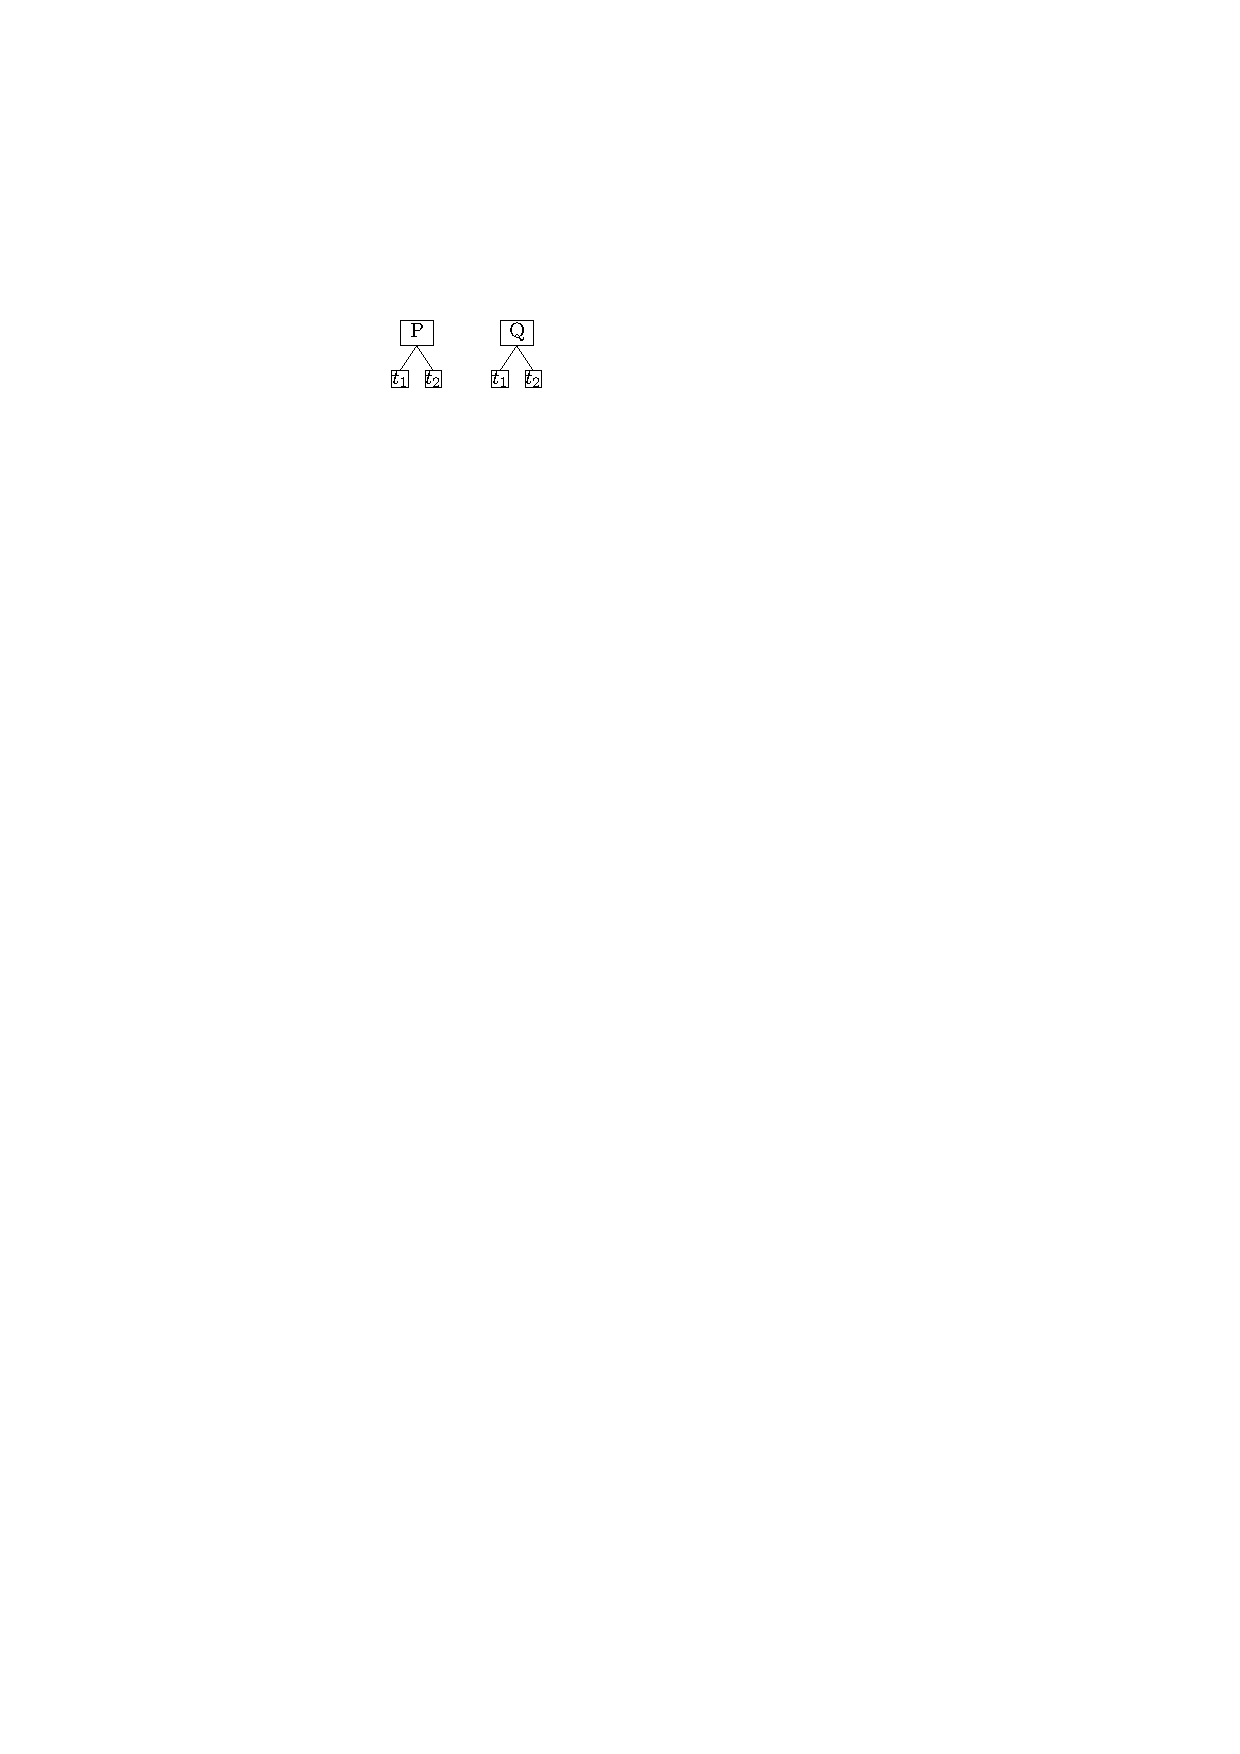
\includegraphics{control_application.pdf}
\end{center}
\caption{system diagram}
\label{sys_dig}
\end{figure}

\textbf{Motivating Example:}
Let us consider two control applications communicating via a common bus to two 
different processors. Each of the control applications has two tasks $T_1$ and $T_2$.
The diagram is given in Fig.\ref{sys_dig}.

The messages transmitted by each of them is denoted by $m_i$,
$m_j$, $m_k$, $m_l$ respectively from P$t_1$, P$t_2$, Q$t_1$, Q$t_2$. To demonstrate the
problem we are considering that the value of $k$ be $6$. We are expecting that invalid message 
can come after $k$ i.e, $6$ valid messages.
\begin{figure}
\begin{center}
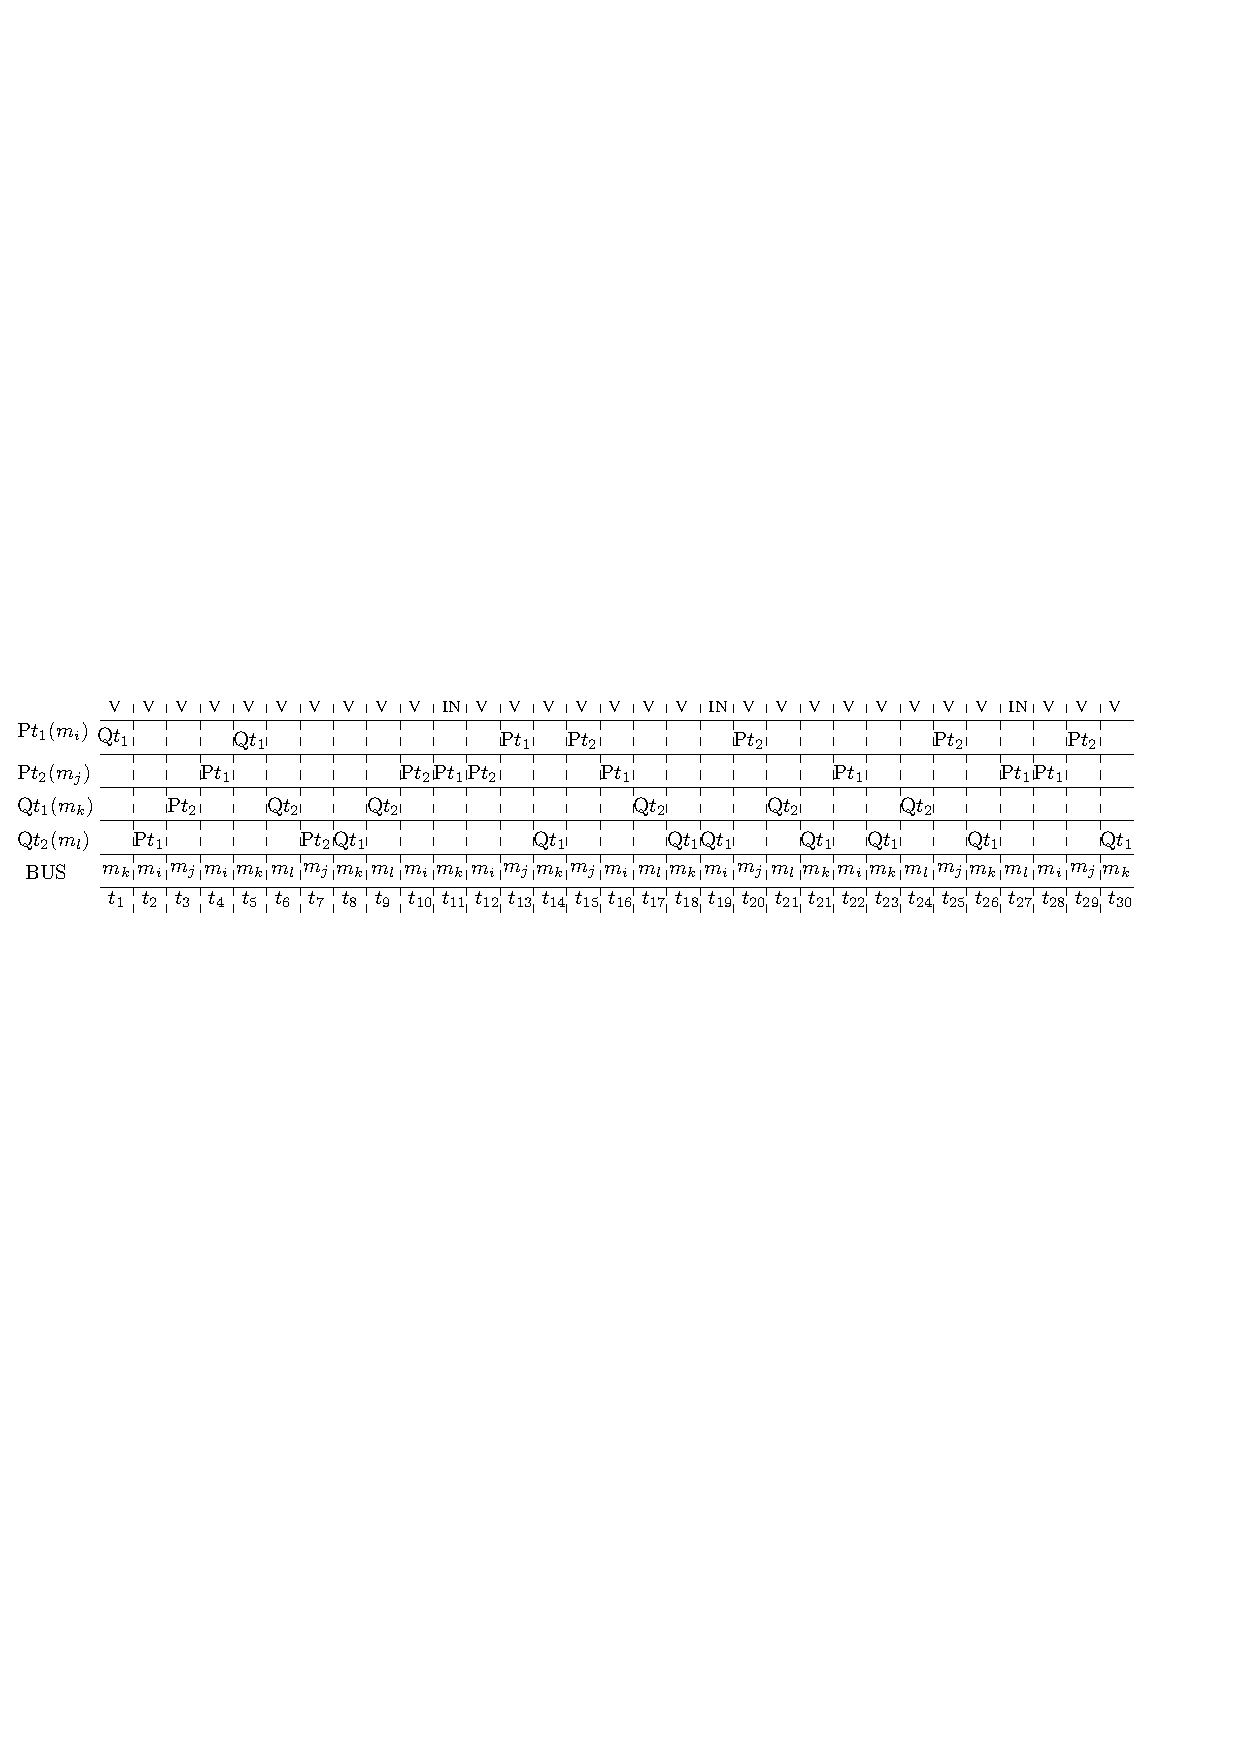
\includegraphics[width=130mm]{prob_1_timing_diagram.pdf}
\end{center}
\caption{Bus timing diagram}
\label{dig1}
\end{figure}

In Fig.\ref{dig1} the timing diagram is given. There are 4 message instances accessing the bus. We are
considering here that P$t_1$ sends message instance $m_i$ and can receive any of the other 
three messages, likewise P$t_2$, Q$t_1$, Q$t_2$ send $m_j$, $m_k$, $m_l$ respectively and will
receive any of the other three messages. 

In the timing diagram the $4$ tasks(two from each control applications) are given vertically with
Bus scheduler and time is plotted horizontally. The timing diagram is basically depicting how the
tasks are receiving messages and whether they are valid or invalid. For a particular task, the 
expected message from the particular task is given at that particular time instant. The Bus scheduler
row shows the message it is receiving. If the received message is not from the expected task then 
it is considered as invalid message otherwise it is valid. For example, let us consider any time 
instant say $t_5$, which says that task P$t_1$ is expecting message from Q$t_1$ and it received
$m_k$ which is message instance from Q$t_1$, so 'V' is written in the upper most row to signify 
a valid message is received. Let us consider another time instant say $t_{11}$ where P$t_2$ is 
expecting P$t_1$ which sends message instance $m_i$. So, $m_i$ was supposed to deliver at time 
instant $t_{11}$ but $m_k$ was delivered which becomes invalid now.'IN' Flag is raised.

\begin{figure}
\begin{center}
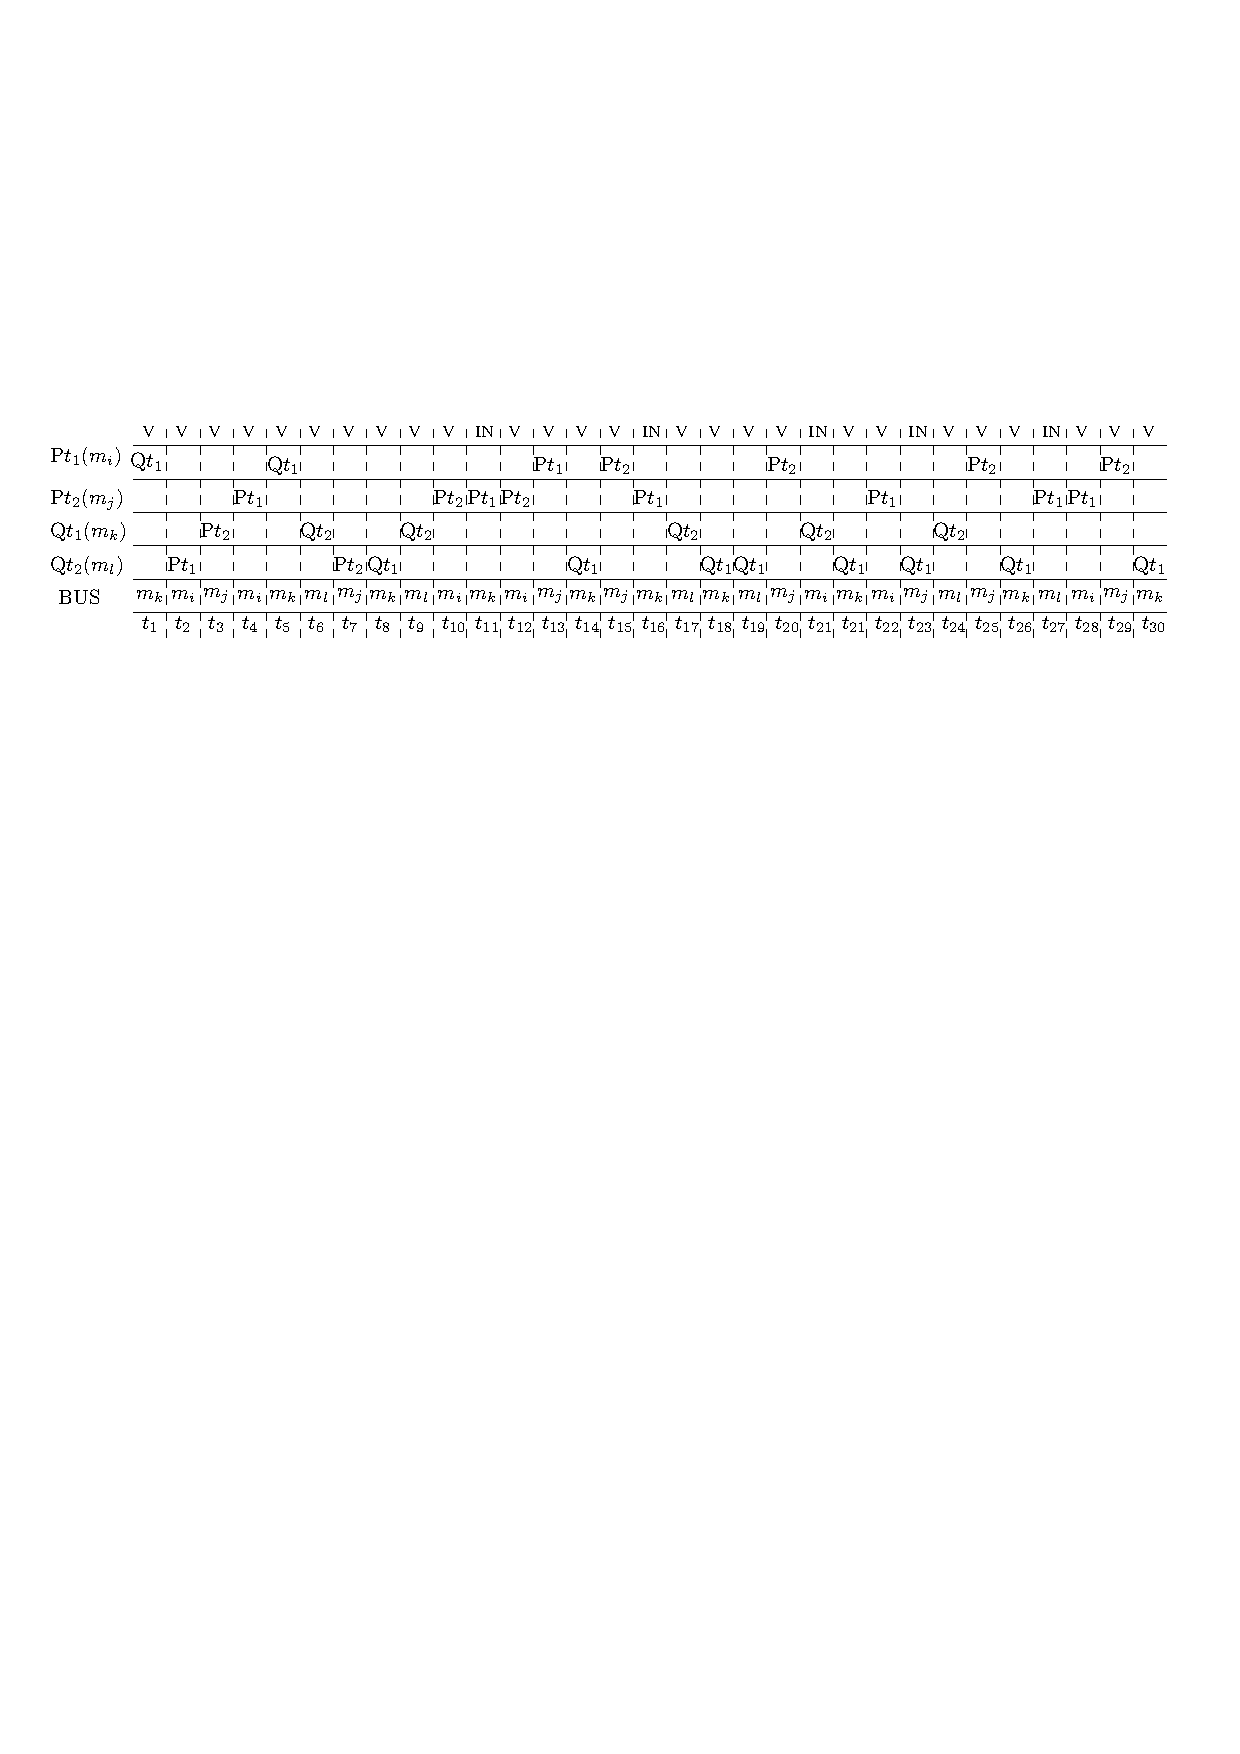
\includegraphics[width=130mm]{prob_1_timing_diagram_2.pdf}
\end{center}
\caption{Bus timing diagram with frequent invalid messages}
\label{dig2}
\end{figure}

In Fig.\ref{dig1} we see that the invalid messages occurred after at least 6 valid messages. Now we can say that
the system is meeting control requirement performance. But in Fig.\ref{dig2} we see that the occurrence of 
invalid messages are not bounded by at least 6 number of messages. In this case we can say that
the system is not meeting the requirement.



